% !TEX root = ../main.tex
% !TEX encoding = UTF-8 Unicode
% !TEX TS-program = pdflatexmk
% !TEX spellcheck = en-US
% !BIB program = biber


% want quotes?
\begin{savequote}[8cm]
Computers are incredibly fast, accurate and stupid; humans are incredibly slow, inaccurate, and brilliant; together they are powerful beyond imagination
%
\qauthor{--- Albert Einstein}
%
\end{savequote}

\chapter{Introduction}\label{ch:1-intro}%
%

% want an abstract per chapter??
\begin{chapterabstract}
  \kant[4]
\end{chapterabstract}

% want a toc per chapter??
\minitoc

% here goes the content
\kant[5]
Some very important \index{Concept}concept is explained here. See \autoref{fig:sample}.

\begin{figure}[htb]
  \centering
  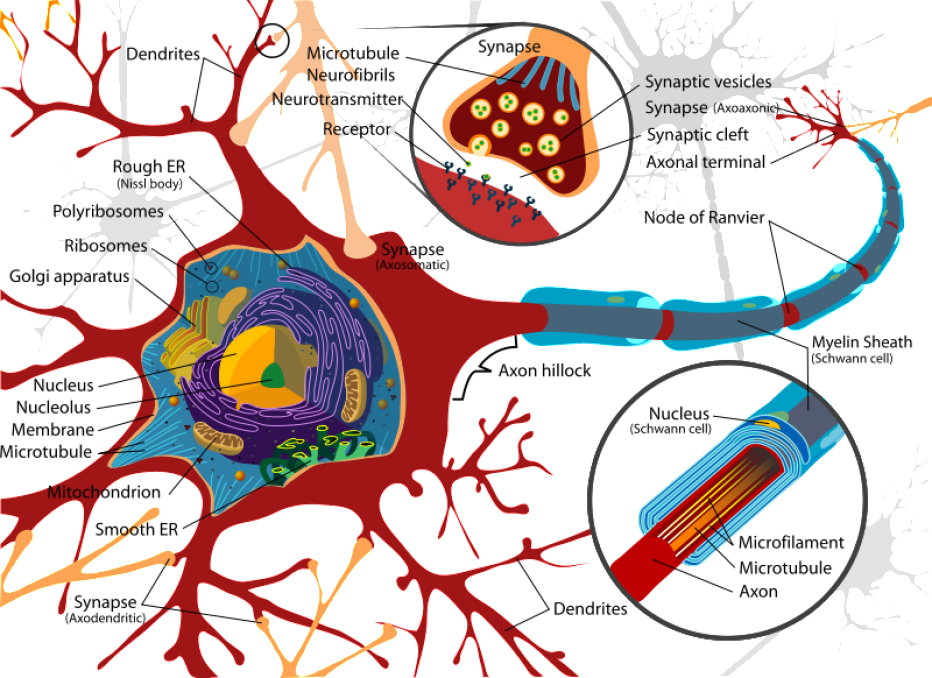
\includegraphics[width=.6\linewidth]{neuron}
  \caption[Some shorter caption for the LOF]{Some potentially very long caption for an image or table.}\label{fig:sample}
\end{figure}

\section{A}
\kant[6-10]

\section{B}
\kant[11]

\subsection{BA}
\kant[12-14]

\subsection{BB}
\kant[14-16]
Some very important \index{Concept}concept is explained again. See \autoref{tab:sample}.

\begin{table}
  \centering
  \begin{tabular}{lll}
    \toprule
     & A & B \\
    \midrule
    C & 1 & 2 \\
    D & 3 & 4 \\
    \bottomrule
  \end{tabular}\caption[shorter caption]{potentially very long caption}\label{tab:sample}
\end{table}

\subsubsection{BBA}
\kant[16-18]

\subsubsection{BBB}
\kant[18-20]

\section{C}
\kant[20-23]

%%%% %%%%%%%%% %%%%%%%%% %%%%%%%%% %%%%%%%%%
%%%%%%%%% %%%%%%%%% %%%%%%%%% %%%%%%%%% %%%%
